\documentclass[11pt,a4paper]{article}

% --- Mathematics (must precede unicode-math) ---
\usepackage{amsmath}
\usepackage{mathtools}

% --- Fonts (lualatex) ---
\usepackage{fontspec}
\usepackage{unicode-math}
\setmathfont{KpMath-Regular.otf}
\setmathfont{KpMath-Bold.otf}[version=bold]

\usepackage{microtype}
\usepackage[dvipsnames]{xcolor}
\usepackage[margin=25mm, top=30mm, bottom=30mm]{geometry}

\usepackage{fancyhdr}
\pagestyle{fancy}
\fancyhf{}
\fancyhead[L]{\small\itshape Polynomial Cubes at a Welded Interface}
\fancyhead[R]{\small\itshape Nestor (2026)}
\fancyfoot[C]{\thepage}
\renewcommand{\headrulewidth}{0.4pt}
\renewcommand{\footrulewidth}{0pt}

\setcounter{secnumdepth}{3}
\usepackage{booktabs}
\usepackage{array}
\usepackage{graphicx}
\usepackage{placeins}
\usepackage[numbers,sort&compress]{natbib}
\usepackage[font=small, labelfont=bf, labelsep=period]{caption}
\usepackage{setspace}
\setstretch{1.15}
\setlength{\parskip}{0.4em}
\usepackage[colorlinks=true, linkcolor=blue!60!black,
            citecolor=blue!60!black, urlcolor=blue!60!black]{hyperref}

% --- Macros ---
\newcommand{\bK}{\mathbf{K}}
\newcommand{\bP}{\mathbf{P}}
\newcommand{\bR}{\mathbf{R}}
\newcommand{\bM}{\mathbf{M}}
\newcommand{\bd}{\mathbf{d}}
\newcommand{\be}{\mathbf{e}}
\newcommand{\bk}{\mathbf{k}}
\newcommand{\bx}{\mathbf{x}}
\newcommand{\bs}{\mathbf{s}}
\newcommand{\bo}{\mathbf{o}}
\newcommand{\balpha}{\boldsymbol{\alpha}}
\newcommand{\bkappa}{\boldsymbol{\kappa}}
\newcommand{\brho}{\boldsymbol{\rho}}
\newcommand{\bxi}{\boldsymbol{\xi}}
\newcommand{\dd}{\mathrm{d}}
\newcommand{\ii}{\mathrm{i}}
\newcommand{\ee}{\mathrm{e}}

\title{\bfseries Coupling Integrals of Polynomial Cubes at a Welded Elastic Interface\\[4pt]
\large The Static Image in Closed Form, and the Plane Waves for the Rest}
\author{T. M. Nestor\\[2pt]\small Independent researcher, Australia}
\date{Draft, 11 October 2026}

\begin{document}
\maketitle

\begin{abstract}
\noindent
In a stratified elastic reference medium the Green's tensor is that of a homogeneous medium plus the waves
reflected and transmitted at the interfaces, and it is most naturally available not as a tabulated function
but through its plane-wave, up- and down-going, factorisation. A volume-integral method that divides the
heterogeneity into cubic cells carrying polynomial fields needs the Galerkin coupling of every pair of
cells through this reference. Between cells in planes that do not touch, the plane-wave representation
with the cells' moments in closed form is exact, and its integral over the lateral wavenumber converges
exponentially. Next to a welded interface it does not: a cell is coupled to itself and to its neighbours
through its own mirror image, which touches them, and the reflected coupling converges only algebraically.
We show that the singular part is the static field of a point force at the interface, to which the
reflected and transmitted kernels tend as $(\omega/\beta q)^2$ at large lateral wavenumber $q$, and obtain it and
its coupling blocks in closed form. Solved in the lateral-wavenumber domain, Rongved's problem gives every
entry as $\ee^{-q\zeta}/q$ times a polynomial; in space the reflected and transmitted static fields are $356$
and $275$ terms built on Kelvin's potential and two logarithmic potentials, Mindlin's terms, which at a
welded interface are present for every pair of distinct media and which we write as a line of images. The
moments of these kernels over a box with the singular point at a vertex reduce, by Euler's identity for
homogeneous functions, to faces, edges and edges to infinity, with Hadamard finite parts where the degree is
negative and two base integrals where it is zero,
$B_1=\tfrac54\mathrm{Cl}_2(\pi/3)-G$ and $B_2=\tfrac13\log[(1+\sqrt2)^2/(2(1+\sqrt3))]$, so that every moment
is elementary apart from Catalan's constant and one value of Clausen's function. The corner moments and
the blocks agree with independent routes to $10^{-15}$ and $10^{-13}$ or better, coincide with the blocks of the homogeneous medium
to $2$ to $8\times10^{-15}$ when the two media are the same, and with the static part subtracted the
plane-wave remainder converges as $Q^{-5}$ in the cutoff $Q$ instead of $Q^{-3}$.
\end{abstract}

% =====================================================================================================
% Paper 4 of the series: 1. the single-site T-matrix of a Legendre cell (LegendreCellTMatrix), 2. the
% coupling between cells in a homogeneous reference (ExactCouplingIntegrals), 3. the error of polynomial
% voxels (PolynomialVoxelError), 4. this paper, split out of Paper 2 (its former section 11) on 11 October 2026.
% =====================================================================================================

\section{Introduction}\label{sec:intro}

A volume-integral method for elastic waves represents a heterogeneous body as a contrast with a reference
medium, divides the contrast into cells, and couples every pair of cells through the Green's tensor of the
reference. When the reference is homogeneous the coupling of cubic cells carrying polynomial fields can be
obtained in closed form and evaluated to round-off \citep{NestorCoupling2026}. In seismology the natural
reference is stratified, and its Green's tensor is that of a homogeneous medium plus waves reflected and
transmitted at the interfaces. The stratified Green's tensor is rarely tabulated: it is computed through its
plane-wave representation, in which, at each lateral wavenumber, waves travel up and down through the layers
and are reflected and transmitted at each interface \citep{FuchsMuller1971,Kennett1983}. A volume method built
on a stratified reference then needs the coupling blocks in a form that uses only this up- and down-going
factorisation \citep{Nestor1996}; tabulating the Green's tensor between all pairs of depths would cost
storage quadratic in the number of depth planes, where the plane waves need only linear storage.

For cells in different planes that do not touch, the plane-wave representation with the cells' moments in
closed form is exact, and its integral over the lateral wavenumber converges exponentially because the
evanescent waves decay between the planes. For cells in touching planes it diverges, and those blocks
are the closed forms of the homogeneous medium \citep{NestorCoupling2026}. At an interface the same failure
reaches further. The reflection of a cell's field is the field of its mirror image, and the image of a cell
that touches the interface touches the cell itself and its neighbours along the interface. The reflected
coupling of every such cell is therefore singular, and its plane-wave integral converges only
algebraically.

This paper removes that obstacle. Its contributions are the following.
\begin{enumerate}
  \item The plane-wave representation of the coupling blocks, stated for the direct, reflected and
  transmitted couplings with the cells' moments in closed form (Section~\ref{sec:planewaves}).
  \item The identification of the singular part of the reflected and transmitted couplings as the static
  field of a point force at a welded interface (Rongved's problem), with the dynamic kernels tending to it
  as $(\omega/\beta q)^2$; subtracting it changes the convergence of the plane-wave remainder from $Q^{-3}$ to
  $Q^{-5}$ (Sections~\ref{sec:planewaves} and~\ref{sec:static}).
  \item The static image and the transmitted static field in space, as $356$ and $275$ canonical terms on
  three potentials, with Mindlin's logarithmic terms written as a line of images (Section~\ref{sec:static}).
  \item The coupling blocks of these fields in closed form: the moments over a box with the singular point at a
  vertex reduce to elementary functions and two constants, $B_1$ and $B_2$, which we evaluate in closed
  form (Sections~\ref{sec:blocks} and~\ref{sec:transmission}).
  \item Verification of each step against routes that share no step with it (Section~\ref{sec:verification}).
\end{enumerate}
The dynamic remainder, smooth by construction, is left to the plane waves; Section~\ref{sec:discussion}
describes how they carry it through a stack of layers.

\section{Cells, blocks and the plane-wave representation}\label{sec:planewaves}

\paragraph{Cells and blocks.} A cell is a cube of half-width $h$ centred at $\bx_c$, with local coordinates
$\bxi=(\bx-\bx_c)/h\in[-1,1]^3$. It carries a nine-component state, the displacement and an independent
engineering strain, as a polynomial in $\bxi$ \citep{NestorLegendre2026}; the field is tested against products
of Legendre polynomials $L_a(\bxi)=\prod_iP_{l_{a,i}}(\xi_i)$, and the source density, the contrast times the
state, is written in the monomials $m_c(\bxi')=\prod_i\xi_i'^{\,e_{c,i}}$. With $\bP(\bx,\bx')$ the
$9\times9$ point propagator of the reference medium, which maps a point source of force and engineering
stress at $\bx'$ to the displacement and engineering strain at $\bx$, a field cell $V_m$ and a source cell
$V_n$ couple through the blocks
\begin{equation}\label{eq:block}
  \bK_{ac}=\int_{V_m}\!\int_{V_n}L_a(\bxi)\,\bP(\bx,\bx')\,m_c(\bxi')\,\dd^3x\,\dd^3x'.
\end{equation}
In a homogeneous medium $\bP$ depends on $\bx-\bx'$ only, and with $\bx=\bx_m+h\bxi$, $\bx'=\bx_n+h\bxi'$ the
block becomes an integral over the separation $\bs=h(\bxi-\bxi')\in[-2h,2h]^3$ against the weight
$W_{ac}(\bs)=\prod_iw_{l_{a,i}e_{c,i}}(s_i)$, with $w_{\alpha\beta}(s)=h\int v^\alpha(v-s/h)^\beta\,\dd v$ the
cross-correlation of the two cells' one-dimensional factors, a piecewise polynomial on eight boxes
\citep{NestorCoupling2026}. The kernel is singular at $\bs=-(\bx_m-\bx_n)$, which for touching cells is a
vertex of some of the boxes.

\paragraph{The plane-wave representation.} Take coordinates in the order $(z,x,y)$, $z$ the depth, and a
lateral wavenumber $\bk=(k_x,k_y)\in\mathbb R^2$, $q=|\bk|$. For each wave $\nu\in\{\mathrm P,\mathrm{SV},\mathrm{SH}\}$
of speed $c_\nu$ ($c_{\mathrm P}=\alpha$, $c_{\mathrm{SV}}=c_{\mathrm{SH}}=\beta$) let
\[
  k_{z,\nu}=\bigl(\omega^2/c_\nu^2-q^2\bigr)^{1/2},\quad\operatorname{Im}k_{z,\nu}\ge0,\qquad
  \bk_\nu^\sigma=(\sigma k_{z,\nu},k_x,k_y),\quad\sigma=\pm1,
\]
the wave vector travelling down ($\sigma=+1$) or up ($\sigma=-1$). Its polarisations are
\[
  \be_{\mathrm P}^\sigma=\frac{\alpha}{\omega}\,\bk_{\mathrm P}^\sigma,\qquad
  \be_{\mathrm{SH}}=\frac{(0,-k_y,k_x)}{q},\qquad
  \be_{\mathrm{SV}}^\sigma=\frac{\beta}{\omega}\,\bk_{\mathrm{SV}}^\sigma\times\be_{\mathrm{SH}},
\]
with $\be_{\mathrm{SH}}=(0,1,0)$ at $\bk=\mathbf 0$. Each is a unit vector in the bilinear sense, $\be\cdot\be=1$,
which, unlike $\be\cdot\bar\be=1$, continues analytically into the evanescent range $q>\omega/c_\nu$. The
state of the wave is the nine-vector $\bd_\nu^\sigma=(\be,\boldsymbol\varepsilon)$ of its displacement and
engineering strain, $\varepsilon_{ij}=\tfrac{\ii}{2}(k_ie_j+k_je_i)$ with $\bk=\bk_\nu^\sigma$ and the three
shears doubled, and $\bM=\operatorname{diag}(1,1,1,1,1,1,\tfrac12,\tfrac12,\tfrac12)$ pairs the
engineering-stress entries of a source with the engineering-strain entries of a state. In a homogeneous
medium of density $\rho$, for $\sigma(z-z')>0$,
\begin{equation}\label{eq:modeprop}
  \bP(\bx,\bx')=\frac{1}{4\pi^2}\int_{\mathbb R^2}\sum_\nu w_\nu\,
  \bd_\nu^\sigma\,\bd_\nu^{\sigma\mathsf T}\bM\,
  \ee^{\ii\bk_\nu^\sigma\cdot(\bx-\bx')}\,\dd^2k,\qquad
  w_\nu=\frac{\ii}{2\rho c_\nu^2k_{z,\nu}},
\end{equation}
the source entering through $\bd_\nu^{\sigma\mathsf T}\bM$ and the field through $\bd_\nu^\sigma$, as reciprocity
requires. For cells in planes that do not touch, $|z_m-z_n|\ge4h$, set $\sigma=\operatorname{sgn}(z_m-z_n)$;
Eq.~\eqref{eq:block} then becomes
\begin{equation}\label{eq:modeblock}
  \bK_{ac}=\frac{1}{4\pi^2}\int_{\mathbb R^2}\sum_\nu w_\nu\,
  \Lambda_a\bigl(\bk_\nu^\sigma\bigr)\,\mu_c\bigl(-\bk_\nu^\sigma\bigr)\,
  \bd_\nu^\sigma\,\bd_\nu^{\sigma\mathsf T}\bM\,
  \ee^{\ii\bk_\nu^\sigma\cdot(\bx_m-\bx_n)}\,\dd^2k,
\end{equation}
with the scalar moments of the two cells, both in closed form for complex arguments \citep{NestorCoupling2026},
\begin{align}
  \Lambda_a(\bkappa)&=h^3\!\int_{[-1,1]^3}\!L_a(\bxi)\,\ee^{\ii h\bkappa\cdot\bxi}\,\dd^3\xi
  =h^3\prod_{i}2\,\ii^{\,l_{a,i}}j_{l_{a,i}}(h\kappa_i),\label{eq:Lambda}\\
  \mu_c(\bkappa)&=h^3\!\int_{[-1,1]^3}\!m_c(\bxi')\,\ee^{\ii h\bkappa\cdot\bxi'}\,\dd^3\xi'
  =h^3\prod_iF_{e_{c,i}}(h\kappa_i),\qquad F_n(t)=\int_{-1}^1\xi^n\ee^{\ii t\xi}\,\dd\xi,\label{eq:mu}
\end{align}
$j_l$ the spherical Bessel functions and $F_n$ a finite combination of them.

\paragraph{Reflection and transmission.} Let medium A, with Lam\'e constants $\lambda_A$, $\mu_A$ and density
$\rho_A$, fill $z<0$ and medium B fill $z>0$, welded at $z=0$ (Figure~\ref{fig:interface}). With the
amplitudes referred to the interface and the polarisations of each medium, a down-going wave $\nu$ in A
gives the up-going wave $\mu$ in A with amplitude $R_{\mu\nu}(\bk)$ and the down-going wave $\mu$ in B with
amplitude $T_{\mu\nu}(\bk)$, obtained at each $\bk$ from the continuity of displacement and traction, a
$6\times6$ linear system \citep{Kennett1983}. For $\bx$ and $\bx'$ both in A the reflected propagator is
\begin{equation}\label{eq:reflected}
  \bP^{R}(\bx,\bx')=\frac{1}{4\pi^2}\int_{\mathbb R^2}\sum_{\mu,\nu}
  \bd_\mu^{A-}\,R_{\mu\nu}\,w_\nu^A\,\bd_\nu^{A+\mathsf T}\bM\,
  \ee^{\ii(\bk_\mu^{A-}\cdot\bx-\bk_\nu^{A+}\cdot\bx')}\,\dd^2k,
\end{equation}
and for $\bx'$ in A and $\bx$ in B the whole coupling is the transmitted one,
\begin{equation}\label{eq:transmitted}
  \bP^{T}(\bx,\bx')=\frac{1}{4\pi^2}\int_{\mathbb R^2}\sum_{\mu,\nu}
  \bd_\mu^{B+}\,T_{\mu\nu}\,w_\nu^A\,\bd_\nu^{A+\mathsf T}\bM\,
  \ee^{\ii(\bk_\mu^{B+}\cdot\bx-\bk_\nu^{A+}\cdot\bx')}\,\dd^2k,
\end{equation}
the superscripts naming the medium whose wave numbers and polarisations are used. The blocks follow as in
Eq.~\eqref{eq:modeblock}, with $\Lambda_a(\bk_\mu^{\pm})\,\mu_c(-\bk_\nu^{+})$ in place of
$\Lambda_a\mu_c$ and the phase $\ee^{\ii(\bk_\mu\cdot\bx_m-\bk_\nu\cdot\bx_n)}$. The vertical phase of the
reflected term is $\ee^{\ii(k_{z,\mu}|z|+k_{z,\nu}|z'|)}$: its decay on the evanescent branch is set by the
distance of the receiver from the source's mirror image $\bx'^*=(-z',x',y')$.

\begin{figure}[t]
\centering
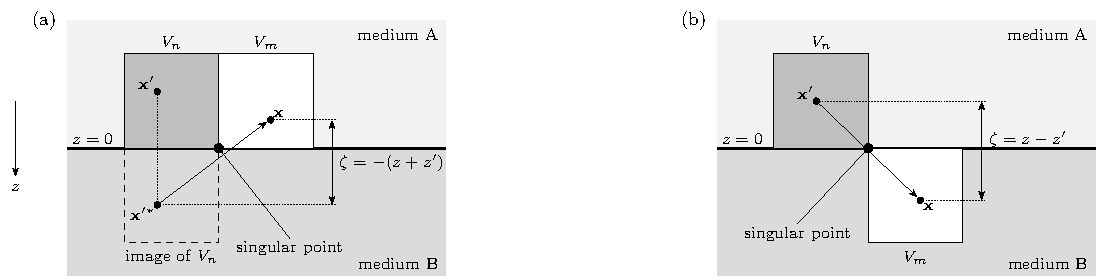
\includegraphics[width=\textwidth]{figures/fig_interface.pdf}
\caption{Cells at a welded interface, in a vertical section; $z$ is depth. (a) Two cells in medium A that
touch the interface and each other. The reflected coupling is the field of the source cell's mirror image
(dashed), at the depth $\zeta=-(z+z')$ below the field point, and the image touches the field cell at the
singular point. (b) A source cell in A and a field cell in B that touch at a point of the interface. The
transmitted coupling depends on $\zeta=z-z'$, and the singular point is where the cells touch.}
\label{fig:interface}
\end{figure}

\paragraph{Where the plane waves fail.} For cells in touching planes, $|z_m-z_n|=2h$, the integral
\eqref{eq:modeblock} does not converge: on the evanescent branch $k_{z,\nu}=\ii\kappa$, $\kappa\to\infty$, the
moments $\Lambda_a$ and $\mu_c$ grow as $\ee^{\kappa h}$ each and cancel the decay $\ee^{-2\kappa h}$ of the
phase. In the reflected coupling the relevant distance is that from the image, $|z_m+z_n|$, which is $2h$
for any two cells that touch the interface, and the same cancellation occurs (Figure~\ref{fig:interface}a).
The integrand then decays only algebraically in $q$, and so does the error of a truncated integral.
Table~\ref{tab:subtraction} shows it for a cell that touches the interface, coupled to its own image: the
change of the integral between successive fourfold cutoffs $Q$ falls by a factor of $68$, close to the
$4^3=64$ of convergence as $Q^{-3}$.

The singular part of the integrand is its behaviour at large $q$. There $k_{z,\nu}=\ii q\,[1-\omega^2/(2c_\nu^2q^2)
+O(q^{-4})]$, and the reflected and transmitted kernels depend on the frequency only through $(\omega/c_\nu
q)^2$. Their limit is the static kernel of Section~\ref{sec:static}, and the difference falls as
$(\omega/\beta q)^2$. Writing $\bK^{R}=\bK^{R}_0+(\bK^{R}-\bK^{R}_0)$, with $\bK^{R}_0$ the block of the static
image, the first term is obtained in closed form (Section~\ref{sec:blocks}) and the second by the
plane-wave integral with the static spectrum subtracted under the integral sign. The remainder converges
as $Q^{-5}$ (Table~\ref{tab:subtraction}), and the same holds for the transmitted coupling.

\begin{table}[h]
\centering
\small
\begin{tabular}{lcc}
\toprule
 & $Qh=10\to40$ & $Qh=40\to160$ \\
\midrule
reflected kernel & $7.5\times10^{-3}$ & $1.1\times10^{-4}$ \\
reflected kernel less its static part & $4.8\times10^{-5}$ & $5.1\times10^{-8}$ \\
\bottomrule
\end{tabular}
\caption{The plane-wave integral of the reflected block of a cell touching the interface, coupled to its own
image: the change between successive fourfold cutoffs of the lateral wavenumber, relative to the block. The
ratios of successive changes, $68$ and $940$, are those of convergence as $Q^{-3}$ and $Q^{-5}$.}
\label{tab:subtraction}
\end{table}

\section{The static field of a point force at a welded interface}\label{sec:static}

\paragraph{In the lateral-wavenumber domain.} Let a unit point force act in A at depth $z'<0$. In the frame
whose $x$ axis lies along $\bk$, the static Navier equations of an isotropic medium have the solutions
$(a+bz)\,\ee^{\pm qz}$, the double root replacing the separate P and S waves of the dynamic problem. The
field in A is Kelvin's field plus a reflected field regular as $z\to-\infty$; the field in B is transmitted
and regular as $z\to\infty$; displacement and traction on the planes $z=\mathrm{const}$ are continuous at
$z=0$. This is the problem of \citet{Rongved1955}, solved here in the lateral-wavenumber domain. Its
solution has a simple structure: every entry of the reflected tensor is $\ee^{q(z+z')}/q$ times a
polynomial of degree at most one in each of $qz$ and $qz'$, and every entry of the transmitted tensor is
$\ee^{-q(z-z')}/q$ times a polynomial in $qz$ and $qz'$, the coefficients rational in the Lam\'e
constants. When the two media coincide the reflected tensor vanishes and the transmitted one is Kelvin's.

\paragraph{In space.} With $\zeta=-(z+z')>0$ for the reflected field and $\zeta=z-z'>0$ for the transmitted
one, $\brho$ the lateral separation and $R=(|\brho|^2+\zeta^2)^{1/2}$, the transform to space follows from
\begin{equation}\label{eq:imagetransform}
  \frac{1}{4\pi^2}\int_{\mathbb R^2}\ee^{\ii\bk\cdot\brho}\,q^{m}\ee^{-q\zeta}\,\dd^2k
  =\begin{cases}(-\partial_\zeta)^{m+1}\Phi_0,&m\ge-1,\\ \Phi_1,&m=-2,\\ \Phi_2,&m=-3,\end{cases}
\end{equation}
with the three potentials
\begin{equation}\label{eq:potentials}
  \Phi_0=\frac{1}{2\pi R},\qquad\Phi_1=-\frac{\log(R+\zeta)}{2\pi},\qquad\Phi_2=\frac{\zeta\log(R+\zeta)-R}{2\pi},
\end{equation}
each the $\zeta$-antiderivative of the one before, $\partial_\zeta\Phi_1=-\Phi_0$ and
$\partial_\zeta\Phi_2=-\Phi_1$. Rotating from the frame of $\bk$ to fixed axes brings factors $k_h/q$; since
$\ii k_h$ becomes $\partial_{\rho_h}$, an entry $(k_h/q)f(q)$ is $\partial_{\rho_h}$ of the transform of
$f/(\ii q)$, and an entry $(k_hk_l/q^2)f(q)$ is $-\partial_{\rho_h}\partial_{\rho_l}$ of the transform of
$f/q^2$. These divisions by $q$ are what produce the powers $m=-2$ and $-3$, and so the logarithmic
potentials. They are the terms that \citet{Mindlin1936} found for the half-space with a free surface; at a
welded interface they are present for every pair of media, with coefficients that vanish only when the
media coincide.

\paragraph{Canonical terms.} The point propagator differentiates the Green's tensor: a receiver derivative
$\partial_z$ acts on the explicit $z$ and on $\zeta$, as $\partial/\partial z-\partial_\zeta$ for the image and
$\partial/\partial z+\partial_\zeta$ for the transmitted field, and similarly for source derivatives and the
lateral ones. Collected, the $9\times9$ static image is a sum of $356$ terms
\begin{equation}\label{eq:imageterms}
  c(\lambda_A,\mu_A,\lambda_B,\mu_B)\;z^{A}z'^{B}\;\partial_{\rho_x}^{\alpha_x}\partial_{\rho_y}^{\alpha_y}
  \partial_\zeta^{\alpha_z}\Phi_j(\brho,\zeta),
\end{equation}
in $61$ families $(j,\balpha)$: $\Phi_0$ with up to four derivatives, and $\Phi_1$ and $\Phi_2$ under lateral
derivatives only (one to four, and two to four), since a $\zeta$-derivative of a logarithmic potential is
the potential below it. The transmitted field has $275$ terms in $46$ families of the same kind. Every kernel
$\partial^{\balpha}\Phi_j$ is homogeneous in $(\brho,\zeta)$, of degree $-1-|\balpha|$, $-|\balpha|$ and
$1-|\balpha|$ for $j=0$, $1$, $2$.

\paragraph{A line of images.} Every logarithmic term carries a lateral derivative and therefore vanishes as
$\zeta\to\infty$. Integrating the relations between the potentials from $\zeta$ to infinity gives
\begin{equation}\label{eq:lineofimages}
  \partial^{\balpha}\Phi_1(\brho,\zeta)=\int_\zeta^\infty\partial^{\balpha}\Phi_0(\brho,t)\,\dd t,\qquad
  \partial^{\balpha}\Phi_2(\brho,\zeta)=\int_\zeta^\infty(t-\zeta)\,\partial^{\balpha}\Phi_0(\brho,t)\,\dd t.
\end{equation}
Mindlin's terms are thus Kelvin's image spread along the vertical half-line beyond the image point, with
uniform and with linearly growing density. This is the form in which their moments are computed.

\section{Coupling blocks with the static image}\label{sec:blocks}

\paragraph{The separation form.} For two cells in A the image kernel depends on the lateral differences
$\rho_h=x_h-x'_h$ but on the vertical sum $\zeta=-(z+z')$. The block is therefore an integral over
$(\rho_x,\rho_y,\zeta)$ against a weight that is a cross-correlation of the cells' factors in the two
lateral coordinates, as in the homogeneous medium, and a convolution in the vertical,
$u_{\alpha\beta}(\tau)=\int v^\alpha(\tau-v)^\beta\,\dd v$ in $\tau=v+v'$, into which the factors $z^A$ and
$z'^B$ of Eq.~\eqref{eq:imageterms} are expanded. The weights are piecewise polynomials with rational
coefficients, computed exactly. The domain divides into boxes on which the weight is a polynomial.

\paragraph{The singular point.} The image kernel is singular only at $\brho=0$, $\zeta=0$, which is reached
when both cells touch the interface and touch each other laterally (Figure~\ref{fig:interface}a), and then at
a vertex of the boxes that hold it. There the vertical weight vanishes as $\zeta^{1+A+B}$, and for every one
of the $356$ terms the integrand is at worst $O(R^{-2})$: it is absolutely integrable, with no distribution
and no derivative to be moved onto the weight. Boxes away from the singular point have smooth integrands
and are integrated by Gauss rules in coordinates centred on each box. On a box with the singular point at
a vertex, reflected onto the positive octant, every term requires the corner moments
\begin{equation}\label{eq:cornermoment}
  M_{j,\balpha}[p,q,r]=\int_0^a\!\!\int_0^b\!\!\int_0^c\rho_x^p\rho_y^q\zeta^r\,
  \partial^{\balpha}\Phi_j(\brho,\zeta)\,\dd\zeta\,\dd\rho_y\,\dd\rho_x,
\end{equation}
with $a=b=c=2h$. They are universal: by homogeneity they scale as a power of $h$ times a number independent
of $h$, the frequency and the media.

\paragraph{Kelvin's potential.} For $j=0$, $\partial^{\balpha}R^{-1}=P_{\balpha}(\brho,\zeta)\,R^{-2|\balpha|-1}$
with $P_{\balpha}$ a homogeneous polynomial of degree $|\balpha|$, so the moments are combinations of the master
integrals
\begin{equation}\label{eq:boxI}
  I[p,q,r;n]=\int_0^a\!\!\int_0^b\!\!\int_0^c x^py^qz^r\,(x^2+y^2+z^2)^{n/2}\,\dd z\,\dd y\,\dd x,
\end{equation}
here for odd $n$ down to $-9$. The integrand is homogeneous of degree $p+q+r+n$ about the singular point,
and Euler's identity with the divergence theorem reduces the box to its three far faces, the faces through
the singular point carrying no flux; on a face the same step in two dimensions reduces to edges, and on an
edge the integral is elementary \citep{NestorCoupling2026}. One transcendental function enters, through the
face integral of $R^{-3}$: $\int_0^b\!\int_0^cR^{-3}\,\dd z\,\dd y=a^{-1}\arctan\bigl(bc/(a\sqrt{a^2+b^2+c^2})\bigr)$
on the face $x=a$, which is continued to lower $n$ by differentiation with respect to $a$.

\paragraph{The logarithmic potentials.} By Eq.~\eqref{eq:lineofimages} the $\zeta$-integral of the box can be
done first, which leaves Kelvin's potential against a polynomial weight in $t$ over the box and over the
semi-infinite column $[0,a]\times[0,b]\times[c,\infty)$ above it. On $[0,c]$ the weight is $t^{r+1}/(r+1)$
($j=1$) or $t^{r+2}/((r+1)(r+2))$ ($j=2$); on the column it is $c^{r+1}/(r+1)$, or
$t\,c^{r+1}/(r+1)-c^{r+2}/(r+2)$. The column is the semi-infinite box less the finite one. Euler's identity
holds on the semi-infinite box, the face at infinity carrying no flux, and its faces reduce to edges that
run to infinity,
\begin{equation}\label{eq:lineinf}
  \int_0^\infty z^r(A^2+z^2)^{n/2}\,\dd z=\tfrac12\,A^{\,r+n+1}\,\mathrm B\Bigl(\tfrac{r+1}{2},-\tfrac{r+n+1}{2}\Bigr),
\end{equation}
Beta functions at half-integers, elementary. Two cases need care. Where the degree $p+q+r+n+3$ of a column
term is negative, each of the two boxes holds an integral that diverges at the singular corner; Euler's
identity then gives Hadamard's finite part of each, and the two finite parts differ by the exact integral
over the column, because their singular contributions at the shared corner are equal. Where the degree is
zero the identity is degenerate, and the column is reduced instead by integration by parts in $t$, then in
$\rho_x$ and $\rho_y$, whose boundary terms are faces at height $c$ and strips at $\rho_x=a$ or $\rho_y=b$,
away from the singular point. Two base integrals remain:
\begin{equation}\label{eq:B12}
  B_1=\int_0^a\!\!\int_0^b\!\!\int_c^\infty R^{-3}\,\dd t\,\dd\rho_y\,\dd\rho_x,\qquad
  B_2=\int_0^a\!\!\int_0^b\!\!\int_c^\infty\rho_x\rho_y\,R^{-5}\,\dd t\,\dd\rho_y\,\dd\rho_x .
\end{equation}

\paragraph{The base integrals.} Both are of degree zero, so they depend only on the ratios of the sides,
which here are equal. The $t$-integrals are elementary, and in polar coordinates $(r,\theta)$ in the
$\brho$-plane so are the radial ones: with $c=1$ and $s=\sqrt{1+r^2}$,
\[
  B_1=\int\!\!\log\frac{1+s}{2}\,\dd\theta,\qquad
  B_2=\int\cos\theta\sin\theta\Bigl[\frac{1}{3s}+\frac23\log(1+s)-\frac13-\frac23\log2\Bigr]\dd\theta,
\]
with $r=\sec\theta$ on $[0,\pi/4]$ and $r=\csc\theta$ on $[\pi/4,\pi/2]$, the two halves equal by symmetry.
For $B_2$ the substitution $v=\cos^2\theta$ makes the remaining integral elementary. For $B_1$ the integral
$2\int_0^{\pi/4}\log\bigl(\tfrac12(1+\sqrt{1+\sec^2\theta})\bigr)\dd\theta$ evaluates to Catalan's constant
$G$, $\pi\log2$, and the imaginary parts of $\mathrm{Li}_2(2^{-1/2}\ee^{\ii\pi/12})$ and
$\mathrm{Li}_2(2^{-1/2}\ee^{7\ii\pi/12})$. Kummer's formula writes $\operatorname{Im}\mathrm{Li}_2(r\ee^{\ii\theta})$
in Clausen functions $\mathrm{Cl}_2(\theta)=\operatorname{Im}\mathrm{Li}_2(\ee^{\ii\theta})$ through the auxiliary
angle $\omega=\arctan\bigl(r\sin\theta/(1-r\cos\theta)\bigr)$ \citep{Lewin1981}, and at both points $\omega=\pi/6$.
The logarithms then cancel, and with $\mathrm{Cl}_2(\pi/2)=G$ and the duplication formula
$\mathrm{Cl}_2(2\theta)=2\mathrm{Cl}_2(\theta)-2\mathrm{Cl}_2(\pi-\theta)$ at $\theta=\pi/6$,
\begin{equation}\label{eq:B12closed}
  B_1=\tfrac54\,\mathrm{Cl}_2\bigl(\tfrac\pi3\bigr)-G=0.35271\,14138\ldots,\qquad
  B_2=\tfrac13\log\frac{(1+\sqrt2)^2}{2(1+\sqrt3)}=0.02151\,58182\ldots.
\end{equation}
Every corner moment is therefore elementary apart from the two constants $G$ and $\mathrm{Cl}_2(\pi/3)$. All
of them are universal numbers, computed once and stored.

\section{Cells on opposite sides of the interface}\label{sec:transmission}

For a source cell in A and a field cell in B the static coupling is the transmitted field, the whole of it,
with no direct part. Its potentials are those of Eq.~\eqref{eq:potentials} with $\zeta=z-z'=|z|+|z'|$, and the
singular point is where the two cells touch at the interface (Figure~\ref{fig:interface}b). The $275$
canonical terms are integrable at that point, as the image's are. In the separation form the vertical
weight is now a cross-correlation in $v-v'$, like the lateral ones, and the corner moments are those of
Section~\ref{sec:blocks}.

The other arrangements follow by symmetry. A field cell in A with a source in B, and two cells in B, are
the problems above reflected in the plane $z=0$ with the two media exchanged. Under the reflection the
displacement $u_z$ and the shear strains $\gamma_{zx}$, $\gamma_{zy}$ change sign, so the block is conjugated
by $\operatorname{diag}(-1,1,1,1,1,1,1,-1,-1)$ in the order $(u_z,u_x,u_y,\varepsilon_{zz},\varepsilon_{xx},
\varepsilon_{yy},\gamma_{xy},\gamma_{zx},\gamma_{zy})$, and each cell polynomial is multiplied by $(-1)$ to
its power of $\xi_z$.

\section{Verification}\label{sec:verification}

Each step was checked against a route that shares no step with it; Table~\ref{tab:verification} collects the
results. The media are A with $\alpha=5.0$, $\beta=3.0$\,km\,s$^{-1}$, $\rho=2.5$\,g\,cm$^{-3}$ and B with
$\alpha=6.5$, $\beta=3.6$\,km\,s$^{-1}$, $\rho=2.8$\,g\,cm$^{-3}$, and $h=0.05$\,km. Errors are relative to
the largest entry of the quantity compared, and the corner moments are measured on the scale $2^{p+q+r}$ of
each monomial.

The checks are of four kinds. The spectral solutions were derived independently in two computer-algebra
systems, and their spatial forms were compared with direct two-dimensional Fourier integration of the
spectral kernels. The corner moments were compared with three routes: Euler's reduction with Gauss rules on
the far faces, tanh-sinh quadrature of the singular volume integral itself, and an evaluation at thirty
digits that integrates one coordinate exactly and then the other two with Duffy coordinates at the corner
\citep{Duffy1982}. We note that adaptive three-dimensional cubature applied directly with the singular point
at a corner, or over the semi-infinite column, can report convergence while in error by as much as
$5\times10^{-7}$, which is why the references integrate one coordinate exactly. The blocks of cells away from
the singular point were compared with a tensor Gauss rule over both cells of the canonical kernel, which
shares neither the separation form nor the exact weights. Two limits close the chain: for identical media
the transmitted blocks must be the touching blocks of the homogeneous medium \citep{NestorCoupling2026},
computed by an unrelated method, and the image must vanish; and the touching block of a cell with its own
image must be the limit of the plane-wave integral \eqref{eq:reflected} of the static spectrum as the
cutoff grows.

\begin{table}[t]
\centering
\small
\setlength{\tabcolsep}{4pt}
\begin{tabular}{p{0.40\textwidth}p{0.30\textwidth}l}
\toprule
quantity & compared with & agreement \\
\midrule
\multicolumn{3}{l}{\emph{Plane-wave representation}}\\
integrand of Eq.~\eqref{eq:modeprop} & residue form of the plane-to-plane kernel & $3\times10^{-15}$ \\
blocks \eqref{eq:modeblock}, planes not touching & closed-form blocks \citep{NestorCoupling2026} & $2$--$6\times10^{-13}$ \\
\midrule
\multicolumn{3}{l}{\emph{Static image}}\\
reflected spectral tensor & second computer-algebra derivation & $5\times10^{-16}$ \\
dynamic reflected kernel, $\omega/\beta q\to0$ & static kernel & $\propto(\omega/\beta q)^2$ \\
spatial form & Fourier integral of the spectrum & $7\times10^{-13}$--$1.3\times10^{-12}$ \\
canonical terms \eqref{eq:imageterms} & direct differentiation of the spatial kernel & $3\times10^{-15}$ \\
\midrule
\multicolumn{3}{l}{\emph{Corner moments}}\\
Euler's reduction, $7$ cases, up to $4$ derivatives & tanh-sinh quadrature of the volume integral & $6\times10^{-16}$--$4.8\times10^{-14}$ \\
closed forms, all $53\,352$ moments, monomials to degree $(6,6,8)$ & Euler's reduction with Gauss rules on the faces & $1.2\times10^{-15}$ \\
$13$ moments, all potentials, $3$ degenerate columns & thirty-digit evaluation & $5\times10^{-23}$--$1.6\times10^{-16}$ \\
$B_1$, $B_2$, Eq.~\eqref{eq:B12closed} & forty-digit angular quadrature & $10^{-40}$ \\
\midrule
\multicolumn{3}{l}{\emph{Reflected blocks}}\\
cells away from the singular point, $4$ pairs, degree-one and degree-two fields & tensor Gauss rule over both cells & $3\times10^{-15}$--$8.5\times10^{-15}$ \\
touching blocks, closed-form corner moments, $3$ pairs & Gauss rules on the far faces & $1.8$--$5.3\times10^{-15}$ \\
cell with its own image & static plane-wave integral, $Qh=320$ to $20\,480$ & $7.9\times10^{-6}\to2.3\times10^{-8}$ \\
\midrule
\multicolumn{3}{l}{\emph{Transmitted field and blocks}}\\
transmitted spectral tensor & second computer-algebra derivation & $4.2\times10^{-16}$ \\
spatial form & Fourier integral of the spectrum & $3.9\times10^{-16}$ \\
canonical terms, different media & Fourier integral of the spectrum & $6.6$--$7.8\times10^{-13}$ \\
identical media: face, edge, corner contact; mirrored; degree two & homogeneous-medium blocks \citep{NestorCoupling2026} & $1.9$--$7.6\times10^{-15}$ \\
different media, cells not touching & tensor Gauss rule over both cells & $1.7$--$5.0\times10^{-13}$ \\
\bottomrule
\end{tabular}
\caption{Independent checks. The last entry of each group of blocks is limited by the accuracy of the
comparison route: the Gauss rule over both cells at order $10$ to about $10^{-13}$, and the static plane-wave
integral by its algebraic convergence.}
\label{tab:verification}
\end{table}

Two remarks qualify the table. The touching reflected blocks agree with the face-quadrature route to
$5\times10^{-15}$, but both routes contract the corner moments with the weights expanded in powers about
the singular corner, which in the homogeneous medium costs about one digit at degree two
\citep{NestorCoupling2026}; the only fully independent check of these blocks, the plane-wave integral, is
limited to $2.3\times10^{-8}$ by its own convergence. And with identical media the image vanishes
identically, to the last bit, on both sides of the interface.

\FloatBarrier
\section{Discussion}\label{sec:discussion}

The static image carries the whole singularity of the coupling at a welded interface, and in closed form it
costs no more than the touching blocks of a homogeneous medium: a fixed set of universal corner moments,
contracted with exact rational weights and with coefficients rational in the Lam\'e constants. The dynamic
remainder is smooth, and the plane waves of Section~\ref{sec:planewaves} carry it at a cost that does not
depend on how close the cells are to the interface, since the subtraction has removed what made the
integral converge slowly.

For a stack of layers the same construction applies interface by interface. The singular part of the
reflected and transmitted couplings comes only from the interface that the cells touch, and is the static
image of that interface; reflections from other interfaces reach a cell after travelling at least one layer
thickness and are smooth. The plane-wave representation extends to the stack through the reflection and
transmission matrices of the layered medium, composed by the recursions of the reflectivity method
\citep{FuchsMuller1971,Kennett1983}. The coupling of every cell with every other is then available from the
up- and down-going factorisation alone, without tabulating the stratified Green's tensor, which is the
storage advantage that motivates the approach; a two-way march in depth that applies the volume operator in
this way is the subject of further work.

Two limitations remain. The corner moments are contracted with the weights in the power basis about the
singular corner; the Legendre basis that restores full double-precision accuracy in the homogeneous medium
\citep{NestorCoupling2026} has not yet been applied to the image boxes, and the touching reflected blocks are
correspondingly expected to lose about one digit at degree two. And the closed form of the base integrals
is stated for cubic corner boxes, $a=b=c$, which is all a grid of cubes requires; for unequal sides the
angular integrals are evaluated by quadrature.

\section*{Data availability}
{\sloppy
The Mathematica notebooks and Python scripts that derive and check every result, and the package they
test, are available at \url{https://github.com/tmnestor/MultipleScatteringCalculations}: the static image and
transmitted field, \path{Mathematica/StaticInterfaceImage.wl}, \path{Mathematica/StaticImageSpace.wl} and
\path{Mathematica/StaticInterfaceTransmission.wl}, with their Python twins
\path{scripts/derive_static_interface_image.py}, \path{scripts/derive_static_image_space.py} and
\path{scripts/derive_static_interface_transmission.py}; the canonical terms,
\path{scripts/derive_interface_image_terms.py}; the corner moments and base integrals,
\path{Mathematica/ImageCornerMoments.wl}, \path{scripts/derive_image_corner_moments.py} and
\path{cubic_scattering/image_moments.py}; the blocks, \path{cubic_scattering/interface_image.py}; the
plane-wave representation, reflection and transmission, \path{cubic_scattering/stratified_march.py}; and
the checks of Table~\ref{tab:verification}, \path{scripts/gate_march_modes.py} and
\path{scripts/gate_interface_image.py}.\par}

\section*{Acknowledgments}
This work began thirty years ago in the author's doctoral research at the Research School of Earth
Sciences of the Australian National University, Canberra \citep{Nestor1996}.

\section*{Declaration of generative AI and AI-assisted technologies in the manuscript preparation process}
\paragraph{Software development.} Software development followed a human-directed, AI-assisted
workflow. The author designed the software originally, but only directed and validated recent
improvements, which build on the author's original Fortran implementation (the
\href{https://github.com/tmnestor/MultipleScatteringCalculations/tree/main/PhD_fortran_code}{\texttt{PhD\_fortran\_code}}
folder of the repository given under Data availability) and an extensive library of Mathematica notebooks,
developed and extended since 1992, that carry out and verify the symbolic derivations; an agentic coding
assistant (Anthropic Claude) operated under human-in-the-loop supervision to implement specified changes and
diagnostic tests. The design, the choice of numerical methods, and the resolution of the principal
technical difficulties were the author's. All AI-generated changes were subject to code review by the
author and validated by automated tests and independent checks.

\paragraph{Manuscript preparation.} During the preparation of this work, the author used Claude
(Anthropic) in order to search for relevant open-access research, to write the TikZ code of the diagrams
and to help redraft the paper into more coherent sections for readability. After using this tool, the
author reviewed and edited the content as needed and takes full responsibility for the content of the
published article.

\bibliographystyle{unsrtnat}
\bibliography{references}

\end{document}
